% questions.tex —— 2000 年·上海卷·文科 · 题目内容片段（无答案）
% 由 tools/generate_projects.py 依来源总账自 2000/2000_数学真题_上海文_试题.md 生成，勿手改（改源 MD 后重跑）


\begin{gktip}
\textbf{来源说明}：固定 PDF 第 1 页题签自题“2000 普通高等学校招生考试（上海卷文）”。当前固定 PDF 仅见两页题面，没有答案、解析或评分页。题面转录以固定原页为准；文字层只辅助定位，不代表内容已核。发布者、出版物、版次、来源链及官方身份未核，仅作本库内部固定字节绑定，来源身份未认证；\texttt{official_answer} 保持 \texttt{null}。

\textbf{图稿说明}：Q8、Q11、Q18、Q20 的图像已按固定原页重绘为 TikZ 矢量源；各图链接位于相应题目后。Q18 仅示拓扑关系，不据示意透视推断题干未给出的长度、角度或垂直关系。
\end{gktip}

\gkpart{一、填空题}

\begin{question}
\gkti{1}已知向量 $\overrightarrow{OA}=(-1,2)$、$\overrightarrow{OB}=(3,m)$，若 $\overrightarrow{OA}\perp\overrightarrow{OB}$，则 $m=\underline{\qquad}$。

\end{question}
\begin{question}
\gkti{2}函数 $y=\log_{2}\dfrac{2x-1}{3-x}$ 的定义域为 $\underline{\qquad}$。

\end{question}
\begin{question}
\gkti{3}圆锥曲线 $\dfrac{(x-1)^2}{16}-\dfrac{y^2}{9}=1$ 的焦点坐标是 $\underline{\qquad}$。

\end{question}
\begin{question}
\gkti{4}计算：$\displaystyle\lim_{n\to\infty}\left(\dfrac{n}{n+2}\right)^n=\underline{\qquad}$。

\end{question}
\begin{question}
\gkti{5}已知 $f(x)=2^x+b$ 的反函数为 $f^{-1}(x)$，若 $y=f^{-1}(x)$ 的图象经过点 $Q(5,2)$，则 $b=\underline{\qquad}$。

\end{question}
\begin{question}
\gkti{6}根据上海市人大十一届三次会议上的市政府工作报告，1999 年上海市完成 GDP（GDP 是指国内生产总值）4035 亿元，2000 年上海市 GDP 预期增长 9\%，市委、市府提出本市常住人口每年的自然增长率将控制在 0.08\%。若 GDP 与人口均按这样的速度增长，则要使本市年人均 GDP 达到或超过 1999 年的 2 倍，至少需 $\underline{\qquad}$ 年。

按：1999 年本市常住人口总数约 1300 万。

\end{question}
\begin{question}
\gkti{7}命题 A：底面为正三角形，且顶点在底面的射影为底面中心的三棱锥是正三棱锥。命题 A 的等价题 B 可以是：底面为正三角形，且 $\underline{\qquad}$ 的三棱锥是正三棱锥。

\Needspace{0.4\textheight}
\end{question}
\begin{question}
\gkti{8}设函数 $y=f(x)$ 是最小正周期为 2 的偶函数，它在区间 $[0,1]$ 上的图象为如图所示的线段 $AB$，则在区间 $[1,2]$ 上 $f(x)=\underline{\qquad}$。
\nopagebreak[4]
\begin{center}% Source: src-8d14b1f9f511665ea10dbda45959a3b445a17806415be6b034f816bec663d7f5
% PDF SHA-256: 35e5d6f6bf052fcd9a2b91a1aa4215766fd4121425cfec7a62cfc4cdc7ab02a1
% PDF page 1, printed page 72, question 8. Only the printed segment and labels are shown.
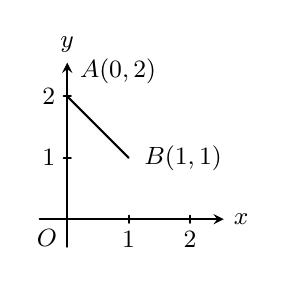
\begin{tikzpicture}[x=0.78cm,y=0.78cm,line cap=round,line join=round,line width=0.65pt,>=stealth,font=\small]
  \draw[->] (-0.45,0) -- (2.55,0) node[right] {$x$};
  \draw[->] (0,-0.45) -- (0,2.55) node[above] {$y$};
  \draw (-0.06,1) -- (0.06,1) node[left=2pt] {$1$};
  \draw (-0.06,2) -- (0.06,2) node[left=2pt] {$2$};
  \draw (1,-0.06) -- (1,0.06) node[below=2pt] {$1$};
  \draw (2,-0.06) -- (2,0.06) node[below=2pt] {$2$};
  \node[below left] at (0,0) {$O$};
  \draw[thick] (0,2) -- (1,1);
  \node[above right=1pt] at (0,2) {$A(0,2)$};
  \node[right=2pt] at (1,1) {$B(1,1)$};
\end{tikzpicture}
\end{center}
\nopagebreak[4]
\end{question}
\begin{question}
\gkti{9}在二项式 $(x-1)^{11}$ 的展开式中，系数最小的项的系数为 $\underline{\qquad}$。（结果用数值表示）

\end{question}
\begin{question}
\gkti{10}有红、黄、蓝三种颜色的旗帜各 3 面，在每种颜色的 3 面旗帜上分别标上号码 1、2 和 3。现任取出 3 面，它们的颜色与号码均不相同的概率是 $\underline{\qquad}$。

\Needspace{0.4\textheight}
\end{question}
\begin{question}
\gkti{11}图中阴影部分的点满足不等式组

\nopagebreak[4]
\[
\begin{cases}
x+y\leq 5,\\
2x+y\leq 6,\\
x\geq 0,\quad y\geq 0,
\end{cases}
\]

在这些点中，使目标函数 $k=6x+8y$ 取得最大值的点的坐标是 $\underline{\qquad}$。
\nopagebreak[4]
\begin{center}% Source: src-8d14b1f9f511665ea10dbda45959a3b445a17806415be6b034f816bec663d7f5
% PDF SHA-256: 35e5d6f6bf052fcd9a2b91a1aa4215766fd4121425cfec7a62cfc4cdc7ab02a1
% PDF page 1, printed page 72, question 11. Shaded quadrilateral follows the printed inequalities.
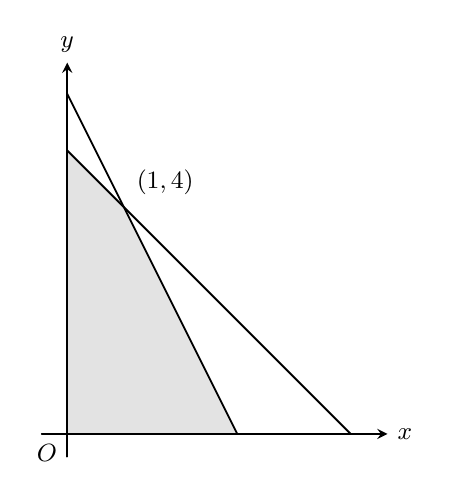
\begin{tikzpicture}[x=0.72cm,y=0.72cm,line cap=round,line join=round,line width=0.65pt,>=stealth,font=\small]
  \fill[gray!22] (0,0) -- (0,5) -- (1,4) -- (3,0) -- cycle;
  \draw[->] (-0.45,0) -- (5.65,0) node[right] {$x$};
  \draw[->] (0,-0.4) -- (0,6.55) node[above] {$y$};
  \draw (0,5) -- (5,0);
  \draw (0,6) -- (3,0);
  \node[below left] at (0,0) {$O$};
  \node[above right=1pt] at (1,4) {$(1,4)$};
\end{tikzpicture}
\end{center}
\nopagebreak[4]
\end{question}
\begin{question}
\gkti{12}在等差数列 $\{a_n\}$ 中，若 $a_{10}=0$，则有等式

\nopagebreak[4]
\[
a_1+a_2+\cdots+a_n=a_1+a_2+\cdots+a_{19-n}\quad(n<19,\ n\in\mathbb{N}^{*})
\]

成立。类比上述性质，相应地：在等比数列 $\{b_n\}$ 中，若 $b_9=1$，则有等式 $\underline{\qquad}$ 成立。

\end{question}
\gkpart{二、选择题}

\begin{question}
\gkti{13}函数 $y=\sin\left(x+\dfrac{\pi}{2}\right)$（$\left[-\dfrac{\pi}{2},\dfrac{\pi}{2}\right]$）是\mbox{（　　）}。

（A）增函数　　（B）减函数　　（C）偶函数　　（D）奇函数

\end{question}
\begin{question}
\gkti{14}设有不同的直线 $a$、$b$ 和不同的平面 $\alpha$、$\beta$、$\gamma$，给出下列三个命题：

① 若 $a\parallel\alpha$，$b\parallel\alpha$，则 $a\parallel b$；

② 若 $a\parallel\alpha$，$a\parallel\beta$，则 $\alpha\parallel\beta$；

③ 若 $\alpha\perp\gamma$，$\beta\perp\gamma$，则 $\alpha\parallel\beta$。

其中正确的个数是\mbox{（　　）}。

（A）0　　（B）1　　（C）2　　（D）3

\end{question}
\begin{question}
\gkti{15}若集合 $S=\{y\mid y=3^x,\ x\in\mathbb{R}\}$，$T=\{y\mid y=x^2-1,\ x\in\mathbb{R}\}$，则 $S\cap T$ 是\mbox{（　　）}。

（A）$S$　　（B）$T$　　（C）$\varnothing$　　（D）有限集

\end{question}
\begin{question}
\gkti{16}下列命题中正确的命题是\mbox{（　　）}。

（A）若点 $P(a,2a)$（$a\neq 0$）为角 $\alpha$ 终边上一点，则 $\sin\alpha=\dfrac{2\sqrt{5}}{5}$。

（B）同时满足 $\sin a=\dfrac{1}{2}$、$\cos a=\dfrac{\sqrt{3}}{2}$ 的角 $a$ 有且只有一个。

（C）当 $|a|<1$ 时，$\tan(\arcsin a)$ 的值恒正。

（D）三角方程 $\tan\left(x+\dfrac{\pi}{3}\right)=\sqrt{3}$ 的解集为 $\{x\mid x=k\pi,\ k\in\mathbb{Z}\}$。

\end{question}
\gkpart{三、解答题}

\begin{question}
\gkti{17}已知椭圆 $C$ 的焦点分别为 $F_1(-2\sqrt{2},0)$ 和 $F_2(2\sqrt{2},0)$，长轴长为 6，设直线 $y=x+2$ 交椭圆 $C$ 于 $A$、$B$ 两点，求线段 $AB$ 的中点坐标。

\Needspace{0.4\textheight}
\end{question}
\begin{question}
\gkti{18}如图所示四面体 $ABCD$ 中，$AB$、$BC$、$BD$ 两两互相垂直，且 $AB=BC=2$，$E$ 是 $AC$ 中点，异面直线 $AD$ 与 $BE$ 所成的角的大小为 $\arccos\dfrac{\sqrt{10}}{10}$，求四面体 $ABCD$ 的体积。
\nopagebreak[4]
\begin{center}% Source: src-8d14b1f9f511665ea10dbda45959a3b445a17806415be6b034f816bec663d7f5
% PDF SHA-256: 35e5d6f6bf052fcd9a2b91a1aa4215766fd4121425cfec7a62cfc4cdc7ab02a1
% PDF page 1, printed page 72, question 18. Schematic topology only; no metric properties are inferred.
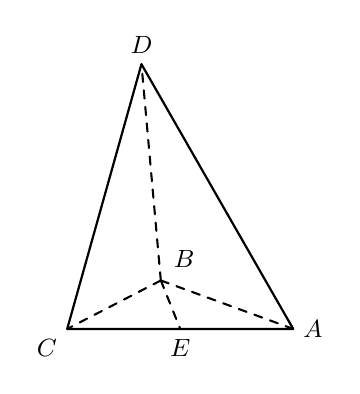
\begin{tikzpicture}[x=0.82cm,y=0.82cm,line cap=round,line join=round,line width=0.75pt,font=\small]
  \coordinate (A) at (3.5,0);
  \coordinate (B) at (1.45,0.75);
  \coordinate (C) at (0,0);
  \coordinate (D) at (1.15,4.1);
  \coordinate (E) at (1.75,0);
  \draw[thick] (C)--(D)--(A)--(C);
  \draw[dashed] (B)--(A) (B)--(C) (B)--(D) (B)--(E);
  \node[above] at (D) {$D$};
  \node[above right=1pt] at (B) {$B$};
  \node[below left] at (C) {$C$};
  \node[right] at (A) {$A$};
  \node[below] at (E) {$E$};
\end{tikzpicture}
\end{center}
\nopagebreak[4]
\end{question}
\begin{question}
\gkti{19}已知函数 $f(x)=\dfrac{x^2+2x+a}{x}$，$x\in[1,+\infty)$。

（1） 当 $a=\dfrac{1}{2}$ 时，求函数 $f(x)$ 的最小值；

（2） 若对任意 $x\in[1,+\infty)$，$f(x)>0$ 恒成立，试求实数 $a$ 的取值范围。

\Needspace{0.4\textheight}
\end{question}
\begin{question}
\gkti{20}根据指令 $(r,\theta)$（$r\geq 0$，$-180^\circ\leq\theta\leq180^\circ$），机器人在平面上能完成下列动作：先原地旋转角度 $\theta$（$\theta$ 为正时，按逆时针方向旋转 $\theta$；$\theta$ 为负时，按顺时针方向旋转 $-\theta$），再朝其面对的方向沿直线行走距离 $r$。

（1） 现机器人在直角坐标系的坐标原点，且面对 $x$ 轴正方向，试给机器人下一个指令，使其移动到点 $(4,4)$；

（2） 机器人在完成该指令后，发现在点 $(17,0)$ 处有一小球正向坐标原点作匀速直线滚动。已知小球滚动的速度为机器人直线行走速度的 2 倍，若忽略机器人原地旋转所需的时间，问机器人最快可在何处截住小球？并给出机器人截住小球所需的指令。（结果精确到小数点后两位）
\nopagebreak[4]
\begin{center}% Source: src-8d14b1f9f511665ea10dbda45959a3b445a17806415be6b034f816bec663d7f5
% PDF SHA-256: 35e5d6f6bf052fcd9a2b91a1aa4215766fd4121425cfec7a62cfc4cdc7ab02a1
% PDF page 2, printed page 73, question 20. Only the coordinate axes and printed ticks are shown.
\begin{tikzpicture}[x=0.22cm,y=0.22cm,line cap=round,line join=round,line width=0.65pt,>=stealth,font=\small]
  \draw[->] (-1.4,0) -- (19.2,0) node[right] {$x$};
  \draw[->] (0,-1.2) -- (0,5.3) node[above] {$y$};
  \draw (4,-0.24) -- (4,0.24) node[below=3pt] {$4$};
  \draw (17,-0.24) -- (17,0.24) node[below=3pt] {$17$};
  \draw (-0.24,4) -- (0.24,4) node[left=3pt] {$4$};
  \node[below left] at (0,0) {$O$};
\end{tikzpicture}
\end{center}
\nopagebreak[4]
\end{question}
\begin{question}
\gkti{21}在 $xOy$ 平面上有一点列 $P_1(a_1,b_1)$、$P_2(a_2,b_2)$、$\cdots$、$P_n(a_n,b_n)$、$\cdots$。对每个自然数 $n$，点 $P_n$ 位于函数

\nopagebreak[4]
\[
y=2000\left(\dfrac{a}{10}\right)^2\quad(0<a<10)
\]

的图象上，且点 $P_n$、点 $(n,0)$ 与点 $(n+1,0)$ 构成一个以 $P_n$ 为顶点的等腰三角形。

\begin{gktip}
\textbf{源文疑点（Q21）}：固定原页印式为 $y=2000\left(\dfrac{a}{10}\right)^2$，本稿照录。按字面该式不含 $x$，与“函数图象上”及后续序列条件的关系异常；在取得可靠同版证据前不改写指数，相关答案保持待核。
\end{gktip}

（1） 求点 $P_n$ 的纵坐标 $b_n$ 的表达式；

（2） 若对每个自然数 $n$，以 $b_n$、$b_{n+1}$、$b_{n+2}$ 为边长能构成一个三角形，求 $a$ 的取值范围；

（3） 设 $c_n=\lg(b_n)$（$n\in\mathbb{N}$）。若 $a$ 取（2）中确定的范围内的最小整数，问数列 $\{c_n\}$ 前多少项的和最大？试说明理由。

\end{question}
\begin{question}
\gkti{22}已知复数 $z_0=1-mi$（$m>0$）、$z=x+yi$ 和 $\omega=x'+y'i$，其中 $x$、$y$、$x'$、$y'$ 均为实数，$i$ 为虚数单位，且对于任意复数 $z$，有 $\omega=\overline{z_0}\cdot\overline{z}$、$|\omega|=2|z|$。

（1） 试求 $m$ 的值，并分别写出 $x'$ 和 $y'$ 用 $x$、$y$ 表示的关系式；

（2） 将 $(x,y)$ 作为点 $P$ 的坐标，$(x',y')$ 作为点 $Q$ 的坐标，上述关系可以看作是坐标平面上点的一个变换：它将平面上的点 $P$ 变到这一平面上的点 $Q$。已知点 $P$ 经该变换后得到的点 $Q$ 的坐标为 $(\sqrt{3},2)$，试求点 $P$ 的坐标；

（3） 若直线 $y=kx$ 上的任一点经上述变换后得到的点仍在该直线上，试求 $k$ 的值。

\end{question}